\documentclass[12pt, paper=a4]{article}
\usepackage[utf8]{inputenc}
\usepackage[german]{babel}
\usepackage{mathrsfs}
\usepackage{amsmath}
\usepackage{amssymb}
\usepackage{listings}
\usepackage{graphicx}
\usepackage{fancyhdr}

\setlength{\parindent}{0pt}

\author{Mareike G\"ottsch, 6695217, Gruppe 2\\Paul H\"olzen, 6673477, Gruppe 1\\Sven Schmidt, 6217064, Gruppe 1}

\title{FGI 2 Hausaufgaben 11}

\rhead{M. G\"ottsch, G-2; P. H\"olzen, G-1; S. Schmidt, G-1}
\pagestyle{fancy}
\begin{document}
\maketitle

\section*{Aufgabe 11.3}
\subsection*{1.}

\begin{figure}[h!]
\centering
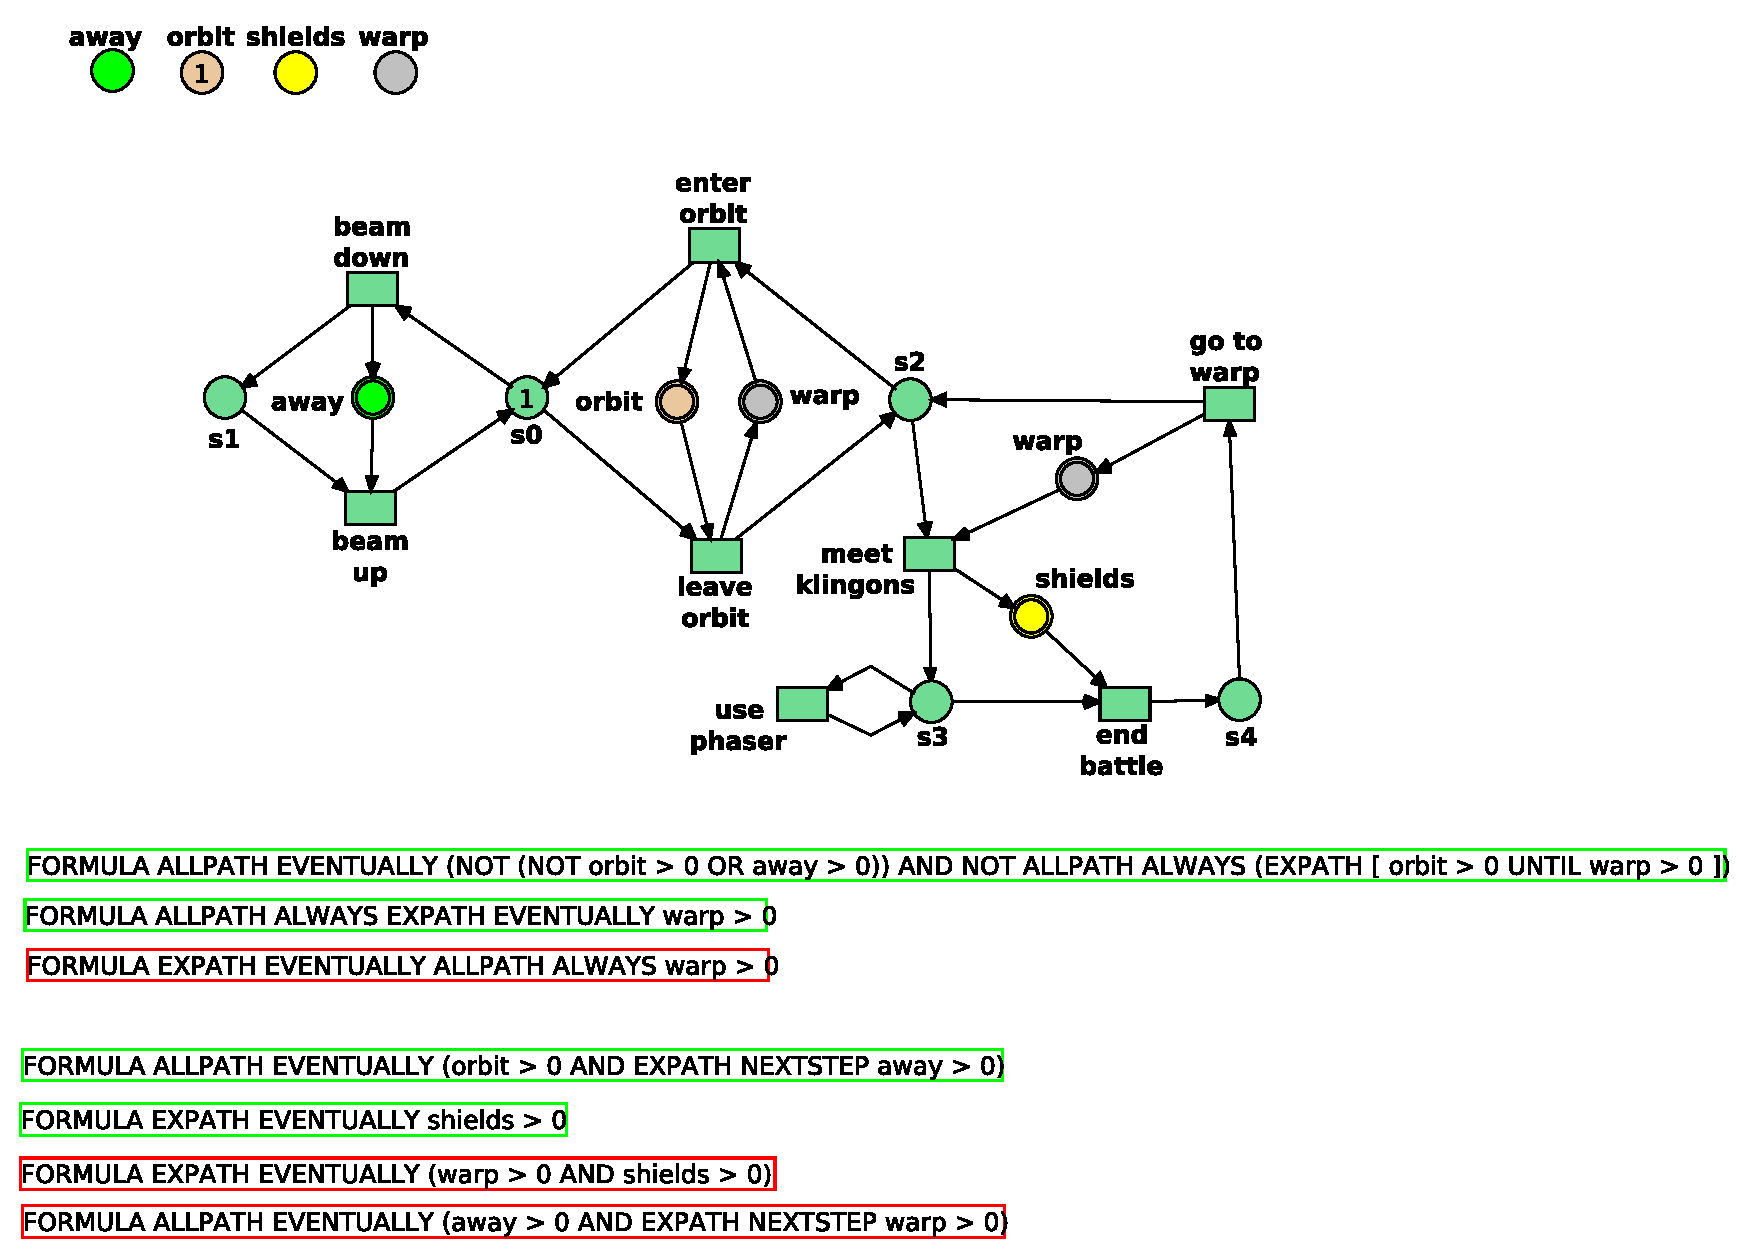
\includegraphics[scale=0.7]{EnterprisePT.pdf}
\caption{PT-Netz mit virtuellen Plätzen zum $TS_{Enterprise}$ aus Aufgabe 5.3}
\end{figure}

\section*{Aufgabe 11.5}
\begin{itemize}
	\item Ein mehrfach gezeichneter Endzustand bezeichnet immer nur ein einziges Objekt. \\
		Wahr oder falsch?\\
		\textit{(Lesestoff Woche 11, Teil 1)}
	\item Der PAP-Kalk\"ul ist korrekt und vollst\"andig, d.h. \(s = t \Leftrightarrow s \overleftrightarrow{\underline{\quad}} t\).\\
		Wahr oder falsch?\\
		\textit{(Lesestoff Woche 11, Teil 1)}
\end{itemize}

\end{document}